%!TEX root = ../thesis.tex

\section{第1章の導入}

運動学を導出し適用するだけでは,ロボットを適切に動作させることができない.
制御をするには人間が意図したとおりに動いてほしい.そのために用いられる方法が軌道計画(経路計画)と軌道生成である.
運動学だけでは適切に動作させることができないというのは,運動学はロボットが出す各時刻の力しか計算できないからである.
今回扱う軌道生成では各時刻の力ではなく,連続した時間の力を計算することができる.これによりロボットに連続的な動作をさせることができる.
その上で,ロボットが障害物などを回避し,ある地点から目的の地点までの軌道を決定するのが軌道計画(経路計画)である.

軌道計画(経路計画)と軌道生成には大きな違いがある.その違いについて,使用される英単語の違いから見ていく.
その後に経路計画と軌道生成についての解説を行う.
\newpage

\begin{figure}[hbtp]
  \centering
 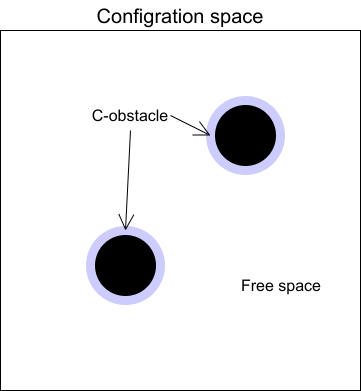
\includegraphics[keepaspectratio, scale=0.8]
      {images/png/ConfigrationSpace.drawio.png}
 \caption{Configration space}
 \label{Fig:ConfigrationSpace}
\end{figure}

経路計画では基本的にコンフィグレーション空間を使用する.
コンフィグレーション空間内にある障害物をC-obstacleと呼ぶ.
C-obstacleは実際の空間の障害物に対応しており,
障害物のギリギリに経路が計画されるのを防ぐため,
Fig.\ref{Fig:ConfigrationSpace}の水色の円のように実際の大きさよりも膨張させて用いられることが多い.

\newpage
